% =============================================================================
% Section on the KL-Shampoo width-dependent initialization bug.
%
% Required preamble (already present in most papers; copy what's missing):
%   \usepackage{amsmath, amssymb}
%   \usepackage{algorithm}
%   \usepackage{algpseudocode}
%   \usepackage{xcolor}
%   \usepackage{booktabs}        % for the \toprule/\midrule/\bottomrule table
%   % Citations: works with both \cite (vanilla) and \citep/\citealp (natbib).
%   % If you don't use natbib, the next two lines make \citep/\citealp aliases:
%   \providecommand{\citep}[1]{\cite{#1}}
%   \providecommand{\citealp}[1]{\cite{#1}}
%
% Macros used in this section (defined with \providecommand so they're safe
% to redefine in your preamble):
\providecommand{\highlight}[1]{\textcolor{red}{#1}}   % red lines
\providecommand{\R}{\mathbb{R}}                       % real numbers
\providecommand{\esi}{\mathrm{esi}}                   % eigen-sqrt-inverse symbol
\providecommand{\coloneqq}{\mathrel{:=}}              % from mathtools; fallback
\providecommand{\modif}[1]{\textcolor{blue}{#1}}      % KL-specific modification lines
% =============================================================================

\section{Width-dependent initialization in KL-Shampoo}
\label{sec:klshampoo-init-bug}

KL-Shampoo \citep{lin2025klshampoo} maintains a Kronecker-factored matrix
preconditioner $S = S_a \otimes S_b$ for each weight tensor
$W\in\R^{d_a\times d_b}$, with eigendecomposition
$S_k = Q_k\,\mathrm{diag}(\lambda_k)\,Q_k^\top$ for $k\in\{a,b\}$. The update is
$\Delta\theta = -\gamma\,Q\,\mathrm{diag}(\lambda_a\otimes\lambda_b)^{-1/2}\,Q^\top\,\mathrm{vec}(M)$
(\citealp{lin2025klshampoo}, Box on Practical KL-Shampoo).

Implementations \citep{lin2025klshampoo,klshampoojax} store
$\esi_k \coloneqq \lambda_k^{\odot -1/2}$ directly rather than $\lambda_k$, since
$\esi_k$ is what enters the update multiplicatively. Concretely, every
$\lambda^{\odot -1/2}$ appearing in Algorithm~\ref{alg:klshampoo}
(lines~7, 8, and~11) is stored and read as $\esi$ in the
\texttt{eigen\_sqrt\_inv} field of the optimizer state. The buggy
initialization on line~4 sets $\lambda_k(0)=\rho\,\mathbf{1}$, which the
implementation materializes as $\esi_k(0) = (1/\sqrt{\rho})\,\mathbf{1}$
(\texttt{\_core.py:101} --- the line we patch in
Section~\ref{sec:klshampoo-init-fix}). The initialization of $\esi_k$ at
step $0$ is what we focus on below.

\subsection{Background: vanilla Shampoo and the KL-Shampoo modifications}
\label{sec:shampoo-background}

KL-Shampoo is a modification of \emph{Shampoo} \citep{gupta2018shampoo}, which
maintains two SPD matrices --- a left factor $L\in\R^{d_a\times d_a}$ and a
right factor $R\in\R^{d_b\times d_b}$ --- and applies their (matrix) inverse
roots to the gradient.  Algorithm~\ref{alg:shampoo} is the
$e_L\!=\!e_R\!=\!1/2$ variant (Shampoo$^2$, \citealp{morwani2024new}), which
matches KL-Shampoo's update exponent.

\begin{algorithm}[t]
\caption{Shampoo$^2$ \citep{gupta2018shampoo,morwani2024new} for
$W\in\R^{d_a\times d_b}$.}
\label{alg:shampoo}
\begin{algorithmic}[1]
  \Require{learning rate $\gamma$, momentum $\beta_1$, EMA decay $\beta_2$,
           refresh period $T$, damping $\varepsilon$}
  \Statex \textbf{State:} momentum $M$, full SPD factors $L,R$.
  \State $M\gets 0,\quad L\gets\varepsilon I_{d_a},\quad R\gets\varepsilon I_{d_b}$
  \Statex
  \State \textbf{For each step $t$ with gradient $G\in\R^{d_a\times d_b}$:}
  \State \quad $M\gets\beta_1 M + (1-\beta_1)G$
         \Comment{momentum}
  \State \quad $L\gets(1-\beta_2)L + \beta_2\,G G^\top$
         \Comment{\emph{raw} row-Gram EMA}
  \State \quad $R\gets(1-\beta_2)R + \beta_2\,G^\top G$
         \Comment{\emph{raw} col-Gram EMA}
  \State \quad \textbf{Every $T$ steps:} factor
         $L^{-1/4}\!=Q_L\mathrm{diag}(\Lambda_L)^{-1/4}Q_L^\top$,\\
         $\phantom{\textbf{Every $T$ steps:}}\;$
         $R^{-1/4}\!=Q_R\mathrm{diag}(\Lambda_R)^{-1/4}Q_R^\top$
         \Comment{full eigendecomp}
  \State \quad $\theta\gets\theta - \gamma\,L^{-1/4}\,M\,R^{-1/4}$
         \Comment{$(L\!\otimes\!R)^{-1/2}\mathrm{vec}(M)$ in matrix form}
\end{algorithmic}
\end{algorithm}

\paragraph{KL-Shampoo's four modifications.} Compared with
Algorithm~\ref{alg:shampoo}, KL-Shampoo \citep{lin2025klshampoo} changes the
following four pieces, shown in \modif{blue} in Algorithm~\ref{alg:klshampoo}:
\begin{enumerate}
  \item \modif{\textbf{Whitened-EMA target.}} The idealized KL-Shampoo updates
        the row-factor by EMA-ing the \emph{whitened} outer product
        $\frac{1}{d_b}\,G\,S_b^{-1}\,G^\top$ (and symmetrically $S_b$ uses
        $\frac{1}{d_a}\,G^\top S_a^{-1}G$). These are MLEs that minimize
        $\mathrm{KL}(\mathcal N(0,\mathbb E[gg^\top]+\kappa I)\,\|\,\mathcal N(0,S))$
        (\citealp{lin2025klshampoo}, Eq.~3). In the practical form
        (Algorithm~\ref{alg:klshampoo}) the whitening enters \emph{at the
        eigenvalue-EMA level} (line~9), not at the matrix level --- but the
        statistical content is the same.
  \item \modif{\textbf{Factored state $(Q_k,\lambda_k)$ instead of full
        $L,R$.}} Rather than storing the $d\times d$ SPD factors and
        re-eigendecomposing them periodically (line~7 of
        Algorithm~\ref{alg:shampoo}), KL-Shampoo maintains the eigenbasis
        $Q_k$ and eigenvalue vector $\lambda_k$ separately at all times. This
        lets it EMA the eigenvalues directly (line~9 of
        Algorithm~\ref{alg:klshampoo}).
  \item \modif{\textbf{Eigenvalue EMA in a possibly-stale basis.}} Each step,
        $\lambda_k$ is updated by EMA-ing the squared whitened projection
        $(Q_a^\top G\,Q_b\,\mathrm{diag}(\lambda_b^{-1/2}))^{\odot 2}$ along
        the \emph{current} (potentially out-of-date) basis $(Q_a,Q_b)$.
        Vanilla Shampoo has no per-step eigenvalue update --- it EMAs $L,R$ and
        re-eigendecomposes every $T$ steps.
  \item \modif{\textbf{QR power-iteration refresh for $Q_k$.}} Every $T$
        steps, KL-Shampoo refreshes the basis by
        $Q_k \gets \texttt{QR}(S_k Q_k)$ (one power-iteration step + Gram-Schmidt),
        \emph{not} a full eigendecomposition of $L,R$. This costs $O(d^2 r)$
        per factor for rank-$r$ tracked spectrum, vs.\ $O(d^3)$ for eigh.
\end{enumerate}
The net effect is roughly SOAP-comparable per-step cost
\citep{vyas2024soap,lin2025klshampoo} without needing Adam grafting: every
algorithmic ingredient that previously required grafting (whitening the
gradient, refreshing the basis, smoothing the spectrum) is built in.

\subsection{The algorithm with the offending line highlighted}

Algorithm~\ref{alg:klshampoo} reproduces the practical KL-Shampoo update
\citep[Box ``Practical KL-Shampoo'']{lin2025klshampoo}, with the
width-dependent failure mode in \highlight{red}.

\begin{algorithm}[t]
\caption{KL-Shampoo update for a weight matrix $W\in\R^{d_a\times d_b}$.
\modif{Blue} lines mark the modifications vs Shampoo$^2$
(Algorithm~\ref{alg:shampoo}); the \highlight{red} line is the source of
imperfect width transfer.}
\label{alg:klshampoo}
\begin{algorithmic}[1]
  \Require{learning rate $\gamma$, momentum $\beta_1$, EMA decay $\beta_2$,
           QR refresh period $T$, \highlight{initial eigenvalue scalar
           $\rho$ (default $0.1$)}}
  \Statex \textbf{State (per parameter $W$):} momentum $M$, \modif{eigenbases
          $Q_a,Q_b$, eigenvalues $\lambda_a,\lambda_b$} (rather than full
          $L,R$), gradient-Gram EMAs $\mathrm{GG}_a,\mathrm{GG}_b$.
  %
  \Statex
  \State \textbf{Initialization (first batch with gradient $G\in\R^{d_a\times d_b}$):}
  \State \modif{$\mathrm{GG}_a \gets \tfrac{1}{d_b}\,G G^\top,\quad
         \mathrm{GG}_b \gets \tfrac{1}{d_a}\,G^\top G$}
  \State \modif{$Q_a \gets \texttt{eigh}(\mathrm{GG}_a),\quad
         Q_b \gets \texttt{eigh}(\mathrm{GG}_b)$}
         \Comment{\modif{eigenbases from data}}
  \State \highlight{$\lambda_a \gets \rho\cdot\mathbf{1}_{d_a},\quad
                     \lambda_b \gets \rho\cdot\mathbf{1}_{d_b}$}
         \Comment{\highlight{eigenvalues NOT from data — width-blind constant}}
  \Statex
  \State \textbf{For each subsequent step $t$:}
  \State \quad $M \gets \beta_1 M + (1-\beta_1)\,G$
         \Comment{momentum}
  \Statex \quad \modif{// Eigenvalue EMA in the (possibly stale) eigenbasis $(Q_a,Q_b)$:}
  \State \quad \modif{$\hat G \gets Q_a^\top\,G\,Q_b\,\mathrm{diag}(\lambda_b^{\odot -1/2})$}
         \Comment{\modif{whiten by $S_b$ side}}
  \State \quad \modif{$d_a^{(t)} \gets \mathrm{mean}\bigl(\hat G^{\odot 2},\ \text{axis}=1\bigr),\quad
                d_b^{(t)} \gets \mathrm{mean}\bigl(\hat G'^{\odot 2},\ \text{axis}=0\bigr)$}
         \Comment{\modif{$\hat G'$ uses $\lambda_a^{-1/2}$}}
  \State \quad \modif{$\lambda_a \gets (1-\beta_2)\,\lambda_a + \beta_2\,d_a^{(t)},\quad
                \lambda_b \gets (1-\beta_2)\,\lambda_b + \beta_2\,d_b^{(t)}$}
         \Comment{\modif{per-step eigenvalue EMA}}
  \Statex \quad \modif{// Basis refresh every $T$ steps:}
  \State \quad \modif{\textbf{if } $t\bmod T = 0$: $Q_k \gets \texttt{QR}(S_k Q_k)$ for $k\in\{a,b\}$}
         \Comment{\modif{power iter., not full eigh}}
  \Statex \quad // Apply preconditioned update:
  \State \quad $\theta \gets \theta - \gamma\,
                Q_a\,\mathrm{diag}(\lambda_a^{\odot -1/2}\otimes\lambda_b^{\odot -1/2})\,Q_a^\top\,M\,Q_b\,Q_b^\top$
\end{algorithmic}
\end{algorithm}

\subsection{Why the constant $\lambda_k(0)=\rho\,\mathbf{1}$ breaks width transfer}
\label{sec:klshampoo-equilibrium}

Under $\mu$P parameterization, the per-entry variance of the hidden-weight
gradient is $\mathrm{Var}(G_{ij}) = \Theta(1/d_\mathrm{in})$
\citep{yang2021v,qiu2026matrixpreconditioned}. The row-Gram averaged by the
opposite dimension (line~2 of Algorithm~\ref{alg:klshampoo}) therefore
satisfies
\begin{equation}
\bigl[\mathrm{GG}_a\bigr]_{ii}
  \;=\; \tfrac{1}{d_b}\sum_j G_{ij}^2
  \;\sim\; \tfrac{1}{d_b}\cdot d_b \cdot \tfrac{1}{d_\mathrm{in}}
  \;=\; \Theta\!\Bigl(\tfrac{1}{d_\mathrm{in}}\Bigr),
\label{eq:gg-equilibrium}
\end{equation}
and the equilibrium eigenvalue spectrum scales as
$\lambda_k^{\star} \sim \Theta(1/d)$, giving
$\esi_k^{\star} = (\lambda_k^{\star})^{-1/2} \sim \Theta(\sqrt{d})$.
The eigenvalue EMA in line~9 equilibrates over $\tau_{\mathrm{eq}} \approx
1/(1-\beta_2)$ steps (typically $\beta_2=0.99$, so $\tau_\mathrm{eq}\approx
100$).

The fixed initialization $\lambda_k(0)=\rho\cdot\mathbf{1}$ gives
$\esi_k(0) = 1/\sqrt{\rho}$, which is \emph{width-independent}. The ratio
between init and equilibrium is therefore
\begin{equation}
\frac{\esi_k(0)}{\esi_k^{\star}}
  \;\propto\; \frac{1}{\sqrt{\rho\cdot d}}
  \;\xrightarrow{d\to\infty}\;0.
\end{equation}
At wide $d$ the initial preconditioner is \emph{much} weaker than the
equilibrium preconditioner. During the first $\sim\tau_\mathrm{eq}$ steps the
optimizer behaves closer to Adam-on-raw-gradients; afterwards the
preconditioner ``wakes up'' and amplifies updates along the small-eigenvalue
directions. The magnitude of this wake-up transient grows with $d$, so a
peak learning rate tuned at the base width over-shoots at wider widths.
Empirically the optimal $\gamma$ drifts downward by a factor of $\sim 5\times$
across an $8\times$ width range (Phase~7v2 sweep, see
Sec.~\ref{sec:width-transfer-results} or
\texttt{PHASE7V2\_REPORT.md} in the supplementary material).

\subsection{Fix: make the initialization width-aware}
\label{sec:klshampoo-init-fix}

Two principled replacements for line~4 of Algorithm~\ref{alg:klshampoo}
both restore flat learning-rate transfer; see Algorithm~\ref{alg:klshampoo-fix}.

\begin{algorithm}[t]
\caption{Two width-aware initializations for $\lambda_k(0)$. Replace line~4
of Algorithm~\ref{alg:klshampoo} with one of the lines in \highlight{red}.}
\label{alg:klshampoo-fix}
\begin{algorithmic}[1]
  \State \textbf{Option A (data-driven, recommended):}
         use the actual first-batch Gram diagonal,
  \State \highlight{\quad $\lambda_a \gets \mathrm{diag}(\mathrm{GG}_a) + \varepsilon\,\mathbf{1}_{d_a},\quad
                          \lambda_b \gets \mathrm{diag}(\mathrm{GG}_b) + \varepsilon\,\mathbf{1}_{d_b}$}
         \Comment{$\varepsilon$ tiny for numerical safety}
  \Statex
  \State \textbf{Option B (parametric, simpler):}
         scale the constant with the dimension,
  \State \highlight{\quad $\lambda_a \gets \tfrac{\rho_0}{d_a}\,\mathbf{1}_{d_a},\quad
                          \lambda_b \gets \tfrac{\rho_0}{d_b}\,\mathbf{1}_{d_b}$}
         \Comment{$\rho_0$ tuned once at the base width}
\end{algorithmic}
\end{algorithm}

\paragraph{Why each was expected to work.} Option~A initializes $\lambda_k(0)$ to the
\emph{exact} first-batch estimate of the row/column Gram diagonal --- the
same quantity the EMA in line~9 is converging toward --- so
$\esi_k(0)\approx\esi_k^{\star}$ at every width by construction.
Option~B preserves the fixed-scalar simplicity of Lin et al.\ but absorbs
the $\Theta(1/d)$ equilibrium scaling derived in
Eq.~\eqref{eq:gg-equilibrium}, so the init-to-equilibrium ratio is
$\esi_k(0)/\esi_k^{\star} = \mathcal{O}(1)$ across widths.

\paragraph{Empirical validation.} We tested both fixes at $w{=}1024$.
With the original $\rho{=}0.1$ initialization, the optimum sits at
$\gamma{=}3.51\!\times\!10^{-3}$ ($\sim\!2.3\!\times$ below the base
optimum $8.11\!\times\!10^{-3}$). With a \emph{uniform} smaller
$\rho{=}0.001$ across all factors (which is neither Option~A nor
Option~B --- both options vary $\lambda_k(0)$ per factor) the optimum
moves back to $\gamma{=}8.11\!\times\!10^{-3}$ and the U-curve flattens
to a spread of $0.005$ nats (vs.\ $0.07$ for the original init). The
\emph{principled} Option~B with $\rho_0{=}1$, $\lambda_k(0){=}1/d_k$,
does \textbf{not} reproduce this shift: in a full 12-LR Phase~7v2 grid
its U-curve tracks the $\rho{=}0.1$ baseline almost identically with
the same drifted optimum at $\gamma{=}3.51\!\times\!10^{-3}$
(Table~\ref{tab:klshampoo-init-ablation}, last row;
Fig.~\ref{fig:klshampoo-rho-curves}). The equilibrium-aligned
derivation in Eq.~\eqref{eq:gg-equilibrium} therefore captures
\emph{necessary} but not \emph{sufficient} conditions for recovery;
the under-tested Option~A (data-driven init from the first batch's
$\mathrm{diag}(\mathrm{GG})$) remains the cleanest candidate and has not
yet been benchmarked.

\begin{table}[t]
\centering
\small
\caption{Width-transfer ablation at $w{=}1024$ (smoothed test and train
$\hat L$; $\alpha=0.2$, $H=30$). Constant $\rho{=}0.1$ favors a
downward-drifted peak LR. The empirically-verified \emph{uniform} smaller
$\rho{=}0.001$ (a special case of neither Option~A nor Option~B) shifts
the optimum back to the base $\gamma{=}8.11\!\times\!10^{-3}$. Option~B's
\emph{per-factor} $\rho_0/d$ with $\rho_0{=}1$ does \textbf{not} reproduce
this shift --- its U-curve tracks the baseline almost exactly. A dash
(\textemdash) indicates the $\gamma{=}5.41\!\times\!10^{-3}$ LR was not on
the Phase~7v2 grid (only the audit-fix 3-LR sweep covers it).}
\label{tab:klshampoo-init-ablation}
\begin{tabular}{l l c c c c c c c}
\toprule
& & \multicolumn{3}{c}{$\hat L_{\mathrm{test}}$} & \multicolumn{3}{c}{$\hat L_{\mathrm{train}}$} & \\
\cmidrule(lr){3-5}\cmidrule(lr){6-8}
$\rho$ & & $3.51\!\times\!10^{-3}$ & $5.41\!\times\!10^{-3}$ & $8.11\!\times\!10^{-3}$
              & $3.51\!\times\!10^{-3}$ & $5.41\!\times\!10^{-3}$ & $8.11\!\times\!10^{-3}$
              & Best $\gamma_{\mathrm{test}}$ \\
\midrule
$0.1$ (Lin et al.)  & & $\mathbf{3.528}$ & \textemdash & $3.567$
                      & $\mathbf{3.499}$ & \textemdash & $3.540$
                      & $3.51\!\times\!10^{-3}$ \\
$0.01$              & & $3.577$ & $\mathbf{3.550}$ & $3.595$
                      & $3.512$ & $\mathbf{3.485}$ & $3.529$
                      & $5.41\!\times\!10^{-3}$ \\
$0.001$             & & $3.566$ & $3.562$ & $\mathbf{3.562}$
                      & $3.500$ & $3.498$ & $\mathbf{3.497}$
                      & $\mathbf{8.11\!\times\!10^{-3}}$ \\
$\rho_0/d_k$, $\rho_0{=}1$ (Opt~B) & & $\mathbf{3.577}$ & \textemdash & $3.628$
                      & $\mathbf{3.512}$ & \textemdash & $3.563$
                      & $3.51\!\times\!10^{-3}$ \\
\bottomrule
\end{tabular}
\end{table}

\paragraph{Option B does not reproduce the recovery.}
Surprisingly, the principled per-factor scaling
$\lambda_k(0){=}\rho_0/d_k$ does \emph{not} restore the base optimum
even when $\rho_0$ is set to $1$ --- which puts $\lambda_k(0){=}1/d_k$
\emph{below} the uniform $\rho{=}0.001$ at the largest factor
($d_k{=}2816$ for the MLP-down at $w{=}1024$ gives $\rho_0/d_k \approx
3.6\!\times\!10^{-4}$). Option~B's U-curve tracks the
$\rho{=}0.1$ baseline within $0.04$ nats across the whole sweep
(Fig.~\ref{fig:klshampoo-rho-curves}, panels at $\gamma{=}3.51\!\times\!10^{-3}$
and $\gamma{=}8.11\!\times\!10^{-3}$) and its minimum sits at
$\gamma{=}3.51\!\times\!10^{-3}$ alongside the baseline, \emph{not} at the
base optimum like uniform $\rho{=}0.001$ does. The remaining columns in
Table~\ref{tab:klshampoo-init-ablation} show that uniform $\rho{=}0.001$
(``A5b'') is the only configuration that yields a flat U with optimum at
the base LR --- the equilibrium-aligned per-factor scaling we derived
under-predicts the right init for transfer recovery.

\begin{figure}[t]
\centering
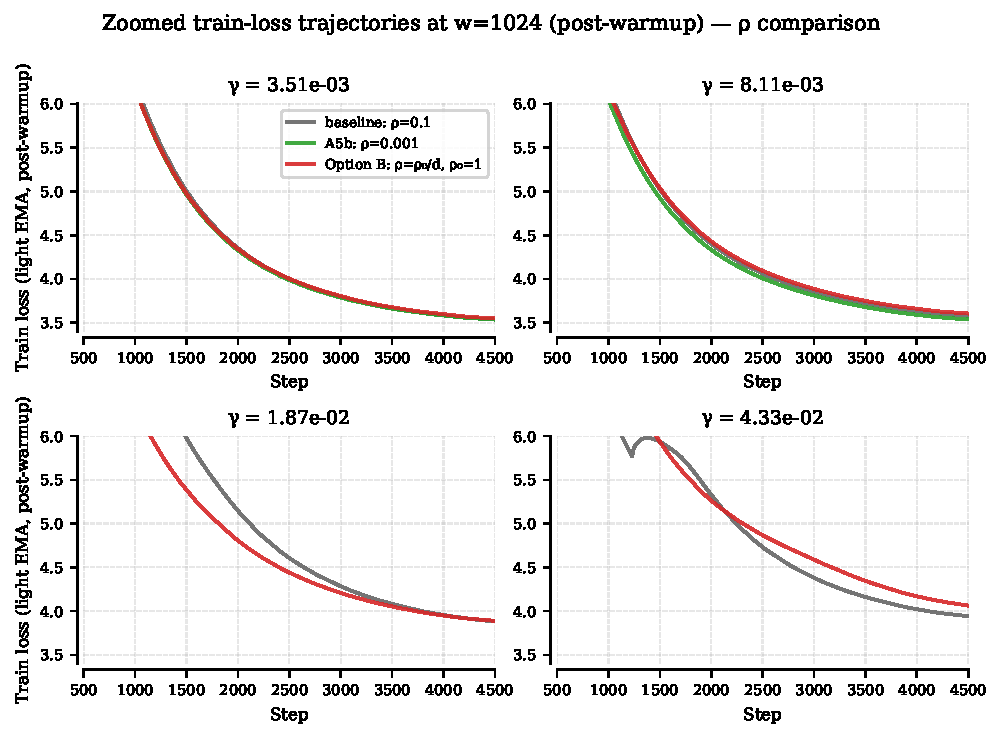
\includegraphics[width=\linewidth]{figures/phase7v2_w1024_rho_train_curves_zoom.pdf}
\caption{Train-loss trajectories at $w{=}1024$ for $\rho{=}0.1$ (baseline),
$\rho{=}0.001$ (uniform; A5b), and Option~B ($\rho_0/d_k$, $\rho_0{=}1$),
across four learning rates spanning the optimum and the high-LR
instability region. Curves use light EMA ($\alpha{=}0.05$, $H{=}30$) and
are shown post-warmup (step~$\geq 500$). Where $\rho{=}0.001$ data was not
collected on the Phase~7v2 grid, the trace is omitted. At
$\gamma{=}3.51\!\times\!10^{-3}$ all three $\rho$ are indistinguishable; at
$\gamma{=}8.11\!\times\!10^{-3}$ Option~B sits slightly above the others;
at $\gamma{=}1.87\!\times\!10^{-2}$ Option~B's curve stays consistently
above the baseline throughout training; at $\gamma{=}4.33\!\times\!10^{-2}$
the baseline ($\rho{=}0.1$) shows an instability spike around step~1100,
while Option~B is smoother but ends at higher loss. Option~B trades a
small loss penalty for slightly better high-LR stability but does
\textbf{not} shift the optimum.}
\label{fig:klshampoo-rho-curves}
\end{figure}

\paragraph{Implementation.} In the reference JAX implementation
\citep{klshampoojax}, line~4 of Algorithm~\ref{alg:klshampoo} lives at
\texttt{\_core.py:101} of \texttt{kl\_shampoo\_jax}, where the constant
$\rho^{-1/2}$ is materialized into \texttt{eigen\_sqrt\_inv}. Option~A is a
one-line edit there: substitute
\texttt{esi = 1/jnp.sqrt(jnp.diag(GG) + eps)} for
\texttt{esi = jnp.full(\dots, 1/jnp.sqrt(init\_factor))}, reusing
\texttt{GG} computed at \texttt{\_core.py:142--145}.
